%----------------------------------------------------------------------------
\chapter{Funkcionális függőség alapú vizsgálatok}
\label{chap:funcDep}
%----------------------------------------------------------------------------

Funkcionális függőségek vizsgálatával először a relációs adatmodell és a relációs adatbázisok tervezése kapcsán kezdtek el foglalkozni.
A relációs adatmodell a \emph{reláció} fogalmára épül -- mely (modell-)entitások valamilyen névvel ellátott kapcsolata --, és ezt egészíti ki a modellen elvégezhető műveletekkel.
Jó példa relációra a \ref{sect:IncQuery}. szekcióban leírt Karate doménünk \textbf{Master} és \textbf{Student} elemei között található \textbf{students} vagy \textbf{master} kapcsolat, de gyakoriak az olyan relációk is, melyek kettőnél több modell elem közötti kapcsolatot reprezentálnak.
Ennek szemléltetésére vegyük példaként egy karate verseny résztvevőit leíró relációt.
A reláció a következő attribútumokat tartalmazza:
\begin{itemize}
\item a versenyző neve (\textbf{Versenyző}),
\item a versenyző mesterének a neve (\textbf{Mester}), és
\item a versenyző dódzsója (\textbf{Dódzsó}).
\end{itemize}
Ennek a relációnak pár sorát láthatjuk a \ref{tab:karateTournamentCompetitorsRelation}. táblázatban.
%
\begin{table}[hbt]
\centering
\tabulinesep=6pt
\caption{Versenyzők adatai\label{tab:karateTournamentCompetitorsRelation}}
\begin{tabu} to \linewidth{|c|c|c|}
\hline
\rowfont{\bfseries}
Versenyző & Mester & Dódzsó \\
\tabucline[1.5pt]{-}
\everyrow{\hline}
\multicolumn{3}{|c|}{\ldots} \\
Bobby Brown & John Kreese & Cobra Kai \\
Daniel LaRusso & Kesuke Miyagi & Miyagi-do Karate \\
Johnny Lawrence & John Kreese & Cobra Kai \\
Jerry Robertson & John Kreese & Cobra Kai \\
\multicolumn{3}{|c|}{\ldots} \\
\end{tabu}
\end{table}
%
A táblázatot közelebbről megvizsgálva láthatjuk, hogy bizonyos mesterek és dódzsók több sorban is szerepelnek, méghozzá párban -- adott mester mellett mindig ugyanaz a dódzsó szerepel.
Ha feltesszük, hogy nincs két ugyanolyan nevű mester és tudjuk, hogy egy mester egyszerre csak egy dódzsóban tanít (a sajátjában), akkor azt mondhatjuk, hogy a \textbf{Mester} attribútum értéke egyértelműen meghatározza a \textbf{Dódzsó} attribútum értékét, vagyis minden olyan sorban, ahol megegyeznek a \textbf{Mester} attribútum értékei, a \textbf{Dódzsó} attribútum értékei is meg fognak egyezni.
Az ezt a jelenséget leíró matematikai konstrukciót nevezzük \emph{funkcionális függőségnek} (vagy függésnek)\cite{Gajdos06}.
Esetünkben azt mondhatjuk, hogy a \textbf{Dódzsó} attribútum funkcionálisan függ a \textbf{Mester} attribútumtól, vagy más szóval, a \textbf{Dódzsó} attribútum értéke származtatható a \textbf{Mester} attribútum értékéből, annak függvénye -- innen jön az elnevezés is.
Ahogyan a függvényeknek is lehet több bemeneti paramétere, úgy funkcionális függőségeknél is előfordul, hogy egy attribútumot több attribútum együttese határoz meg -- gondoljunk csak arra, hogyan befolyásolja egy félév során történt számonkérések eredménye az év végi jegy alakulását egy tantárgyból.
Előfordulhat olyan eset, amikor ugyanaz az egy vagy több attribútum több különböző attribútumot is meghatároz -- az előző példa alapján a számonkérések eredménye nem csak az év végi jegyet határozhatja meg, hanem például hogy mehetünk-e elővizsgára vagy épp pótzárthelyire.

Az előbbi két megfigyelés alapján általánosságban \emph{attribútumhalmazok} közötti funkcionális függőségekről beszélhetünk, és ez az elterjedt matematikai jelölésrendszerben is megjelenik.
Ebben a rendszerben az ,,$X$ attribútumhalmaz meghatározza $Y$ attribútumhalmazt'' kifejezésére az $X \rightarrow Y$ jelölést használjuk.
Legtöbbször ezt a jelölést fogom használni még akkor is, ha a halmazok valamelyike csak egy attribútumot tartalmaz.
Ha kifejezetten egyesével szeretném jelölni az attribútumokat, akkor azokat kisbetűs nevekkel fogom illetni, pl. $x$, $x \in X$.
Két attribútumhalmaz unióját a rövidség kedvéért az attribútumhalmazok juxtapozíciójával\footnote{\emph{juxtapozíció}: egymás mellé helyezés} jelöljük: $X \cup Y \equiv XY$.

Felmerül a kérdés, hogy ha rendelkezünk pár funkcionális függőséggel ($\mathcal F$) egy reláció felett, akkor mi azoknak a függőségeknek a legbővebb halmaza, amely szükségszerűen fennáll $\mathcal F$ következményeképp.
Válaszként Armstrong 1974-ben publikálta azt a három axiómát (pontosabban következtetési szabályt), melyek segítségével generálhatjuk az összes olyan funkcionális függőséget, melyet $\mathcal F$ implikál.
Az axiómák a következőek:
\begin{itemize}
    \item \textbf{reflexivitás}: ha $Y \subseteq X$, akkor $X \rightarrow Y$
    \item \textbf{tranzitivitás}: ha $X \rightarrow Y$ és $Y \rightarrow Z$, akkor $X \rightarrow Z$
    \item \textbf{bővíthetőség}: ha $X \rightarrow Y$, akkor $XZ \rightarrow YZ$
\end{itemize}
Az Armstrong axiómák és tulajdonságaik bővebb tárgyalása megtalálható a \cite{Gajdos06}-ben.

\emph{Triviális függőségnek} nevezzük azt az esetet, amikor egy attribútumhalmaz önmagát határozza meg ($X \rightarrow X$).
Ez a függőség minden esetben teljesül Armstrong reflexivitás axiómája alapján.
Ehhez némileg hasonló az az eset, amikor egy attribútumhalmaz egy konstans értéket határoz meg ($X \rightarrow k$, ahol $k$ egy konstans érték, például $42$ vagy \textit{,,alma''}).
Ez a függőség is bármikor teljesül, hiszen csak azt mondja ki, hogy bármilyen $X$ halmaz mellett a konstans értéke önmaga marad, amely a konstans definíciójából természetesen következik.
Az ilyen függőségek esetén a konstansokat az üres halmazzal ($\varnothing$) szokás reprezentálni, hiszen nem tartalmaznak attribútumot: $X \rightarrow \varnothing$.
Ennek a fordítottja, mikor egy konstans érték határoz meg egy attribútumhalmazt ($k \rightarrow X$ vagy $\varnothing \rightarrow X$).
Ebben az esetben az $X$ halmazban lévő attribútumok értéke is konstans lesz.

\section{Származtatott tulajdonságok}

Aki programozott már valamilyen objektum-orientált paradigmát támogató nyelven, annak minden bizonnyal ismerős az elérőfüggvények fogalma (\emph{getter} és \emph{setter}).
Aki ismer olyan nyelvet, amely támogatja, hogy ezeket a metódusokat a tulajdonság-eléréssel megegyező szintaxist használva érjük el, úgynevezett \emph{property}-ként -- ilyen nyelvek például: \CSharp, D, Delpi, Python --, az tudja milyen hasznos ez a funkcionalitás, melynek segítségével könnyedén illeszthetünk akár komolyabb logikákat egy egyszerű tulajdonság-elérés mellé, vagy ahelyett.
Az objektumok ezen tagjait szokás \emph{származtatott tulajdonságoknak} nevezni.

A származtatott tulajdonságok használatához az alábbi dolgokra van szükség EMF modellek esetén:
\begin{itemize}
    \item az Ecore metamodellen definiálni kell egy \texttt{EAttibute}-ot vagy \texttt{EReference}-t a kívánt névvel, típussal és multiplicitással, és beállítani a következő tulajdonságokat a létrejött \texttt{EStructuralFeature}-ön, hogy annak viselkedése megfelelő legyen: \textbf{derived} = \texttt{true}, \textbf{changeable} = \texttt{false}, \textbf{transient} = \texttt{true}, \textbf{volatile} = \texttt{true}
    \item definiálni kell a származtatás logikáját, és azt hozzárendelni a modellünkhöz
\end{itemize}
A tulajdonságok mögötti logikát a Genmodel metamodellből generált Java forráskódhoz kell hozzáadnunk vagy kézzel, vagy valamilyen eszköz által generáltan.
Az egyik ilyen eszköz maga az EMF-IncQuery, melynek lekérdező nyelvében definiálhatunk egy mintát, amelyet a \texttt{QueryBasedFeature} annotációval megjelölve, a rendszer automatikusan generálja a szükséges kódot a minta alapján a megfelelő helyre. 
Ennek a technikának a részletes leírását a \cite{DerivedFeature} tartalmazza.
Az alábbi kódrészlet a \ref{sect:IncQuery}. szekció Karate modelljéhez definiál egy lekérdezést, amelynek segítségével automatikusan tudjuk biztosítani, hogy egy tanítvány dódzsója megegyezzen a mesterének dódzsójával.
%
\begin{lstlisting}
package karate.incquery

import "http://karate/1.0"

@QueryBasedFeature
pattern dojo(this : Student, result : Dojo) = {
    Student.master.dojo(this, result);
}
\end{lstlisting}
%
A minta neve (\texttt{dojo}) megegyezik a származtatni kívánt tulajdonság nevével.
A minta első paramétere (\texttt{this : Student}) a gazdaobjektum, melyen a származtatott tulajdonság található.
A minta második paraméterébe (\texttt{result : Dojo}) kerül majd maga a tulajdonság értéke -- ezért tekinthetünk rá úgy, mint egy kimeneti változóra, vagy egy függvény végeredményére.
A mintában lévő logika pedig a kapcsolatot írja le a gazdaobjektum és a tulajdonság között.

A fenti kódrészletben az annotáció alapértelmezett beállításait használjuk, ezért kötött a minta neve, és paramétereinek szerepe a pozíciójuktól függ.
Ezek a kötöttségek az annotáció megfelelő paraméterezésével természetesen feloldhatóak.
A \texttt{QueryBasedFeature} annotáció egyik paramétereként megadható a származtatott tulajdonság jellege (\emph{kind}), melynek értéke lehet egyes (\emph{single}), többes (\emph{many}), számláló (\emph{counter}), összeg (\emph{sum}) vagy iteráció (\emph{iteration}), és az alapértelmezett értéke a származtatott tulajdonság metamodellben beállított multiplicitásának megfelelően egyes vagy többes.
A \texttt{QueryBasedFeature} annotáció paraméterezéséről bővebb tájékoztatást a \cite{DerivedFeature} ad.

Karate doménünkben kikötöttük, hogy egy tanítvány egyszerre csak egy dódzsóban tanul, tehát a tanítványok (\textbf{Student}) \textbf{dojo} tulajdonságának multiplicitása egyes.
A domén ezen tulajdonságát a metamodell készítésekor is figyelembe vettem, ahogy az a \ref{fig:karateMetaModel}. ábrán is látható.
Ugyanezt a tulajdonságot tükrözi a fenti mintában található logika is, hiszen a metamodell alapján minden tanítványnak pontosan egy mestere van, és minden mester pontosan egy dódzsóban tanít, tehát minden tanítvány pontosan egy dódzsóban kell hogy tanuljon.
A funkcionális függőség formalizmusát felhasználva a következőket mondhatjuk a tanítvány ($S$), mester ($M$), és dódzsó ($D$) attribútumok kapcsolatáról: a mester attribútum funkcionálisan függ a tanítvány attribútumtól ($S \rightarrow M$), a dódzsó attribútum funkcionálisan függ a mester attribútumtól ($M \rightarrow D$).
Ezekből Armstrong tranzitivitás-axiómáját felhasználva következik, hogy $S \rightarrow D$, vagyis a tanítvány attribútum funkcionálisan meghatározza a dódzsó attribútumot.
Ez, a funkcionális függőség definíciója szerint azt jelenti, hogy ugyanahhoz a tanítványhoz minden esetben ugyanaz a dódzsó fog tartozni, amit úgy is értelmezhetünk, hogy egy tanítvány pontosan egy dódzsóban tanulhat -- ahogyan azt a doménleírásunk alapján vártuk.

Láthatjuk, hogy egy ilyen egyszerű esetben a funkcionális függőség eszközével magából a logikából is meg tudjuk határozni egy származtatott tulajdonság multiplicitását.
Ez azonban komplexebb minták esetén nehézzé vagy akár megoldhatatlanná is válhat, ezért szükséges a multiplicitás manuális beállítása a metamodellen.
Mi történik azonban akkor, ha rosszul álltjuk be ezt az értéket, vagy a logika módosítása után elfelejtjük azt frissíteni?
A legszerencsésebb esetben a modell többes jellegűként definiálja a tulajdonságot, azonban a származtatási logika miatt mindig csak legfeljebb egy érték kerül bele. Más esetekben az egyszerű csonkolástól a várt és kapott értékek típusának eltérése miatti futásidejű kivételig terjedő viselkedést kaphatunk.

\section{Származtatott tulajdonságok multiplicitásának ellenőrzése}

Amint azt az előzőekben szemléltettem, hasznos információkhoz juthatunk az \gls{EMF} modellek és az EMF-IncQuery minták elemzésével a bennük található funkcionális függőségek szempontjából.
Az így kinyert információk segítségével figyelmeztethetjük a felhasználót ha ellentmondást találunk a modell és a logika között, illetve javaslatokat tehetünk a logika információtartalma alapján a modell javítására.
Én, az előző példában is bemutatott, származtatott tulajdonságok jellegének fejlesztési idejű ellenőrzését valósítottam meg egyes és többes jelleg esetén.
%\todo{mi a helyzet a többi jelleggel (counter, sum, iter)? -> főleg típus alapú ellenőrzések}

\subsection{Tervezés}

Az elkészült ellenőrzések mögötti logika megértéséhez előbb nézzük meg, mit is jelent egy származtatott tulajdonság egyes vagy többes jellege funkcionális függőségek szempontjából.
Ha a metamodell egy eleme ($E$) és annak egy tulajdonsága ($A$) között funkcionális függés áll fenn ($E \rightarrow A$), akkor -- definíció szerint -- az elem egy adott egyedéhez mindig ugyanaz az érték fog társulni a tulajdonságban.
Vagyis az említett \emph{függőség fennállása esetén a tulajdonság jellege biztosan egyes}.
Ellenkező esetben arra következtethetünk, hogy a tulajdonság jellege többes.
Ez a következtetés \emph{konzervatív}, vagyis ha esetleg tévednénk, és a függés mégis fennáll -- csak nem sikerült meghatároznunk --, akkor a tulajdonságnak többes jellege ellenére mindig pontosan egy eleme lesz, ami azonban nem vezet hibához.
Tehát ha valahogyan sikerülne szert tennünk az entitás és a tulajdonság közt fennálló funkcionális függőségekre, akkor az ezek alapján számított jelleget összevetjük az Ecore modellben definiált tulajdonságnál manuálisan megadott multiplicitással, és eltérés esetén figyelmeztethetjük a fejlesztőt.
A leírtakat a \ref{tab:funcDepVsModelMulti}. táblázat szemlélteti.
\begin{table}[hbt]
\centering
\renewcommand{\arraystretch}{1.5}
\caption{Funkcionális függőség és tulajdonság multiplicitás közti kapcsolat\label{tab:funcDepVsModelMulti}}
\begin{tabular}{|c|c|c|}
\hline
\diagbox{multiplicitás}{$E \rightarrow A$} & {\renewcommand{\arraystretch}{1}\begin{tabular}{c}nincs\\ (vagy nem\\ eldönthető)\end{tabular}} & van \\
\hline
1 & figyelmeztetés & \checkmark \\
\hline
* & \checkmark & figyelmeztetés \\
\hline
\end{tabular}
\end{table}

Mivel az entitás és a származtatott tulajdonság kapcsolatát esetünkben egy EMF-IncQuery minta, az abban található logika írja le, ezért a keresett funkcionális függőségek is ebben találhatóak.
A feladatunk tehát a \texttt{QueryBasedFeature} annotációval megjelölt minta paraméterei között fennálló funkcionális függőségek felderítése, melyhez szükségünk lesz a minta egyes törzseiben található funkcionális függőségek összegyűjtésére.
A minta egy adott törzse egy vagy több kényszerből áll, melyek logikai ÉS kapcsolatban állnak egymással, tehát ha a mintatörzs illeszkedik, akkor az összes benne lévő kényszer is teljesül.
Emiatt a törzsben fennálló funkcionális függőségek halmaza a törzsben található kényszerek által egyenként meghatározott funkcionális függőséghalmazok uniója.
Járjuk hát végig az előforduló kényszertípusokat, melyik milyen funkcionális függéseket rejt a paramétereire nézve.

Funkcionális függőségek szempontjából a legegyszerűbben elemezhető kényszer a \textbf{típuskényszer}.
Mivel ez a kényszer egyetlen paraméterének egyedül a típusát határozza meg, ami -- az egyke (singleton) típusokat kivéve -- nem határoz meg funkcionális függőséget.
Az egyke típusok felismeréséhez szükséges kardinalitás információt a rendszer sajnos nem szolgáltatja, így ezt nem tudtam kihasználni a függőségek összegyűjtésekor.

Második a sorban az \textbf{összehasonlítás kényszer}, mely két paraméterének egyenlőségét vagy egyenlőtlenségét mondja ki.
Míg egyenlőség esetén a két paraméter ($X$ és $Y$) kölcsönös függésben áll ($\left\{ X \rightarrow Y , Y \rightarrow X \right\}$), addig egyenlőtlenség esetén semmilyen függőséget nem tudunk meghatározni a kettő közt.

Kényszer paramétere általánosságban bármilyen kifejezés lehet.
Mivel mi a változók közötti függőségeket szeretnénk megállapítani, ezért kifejezések közötti függőség alatt valójában a kifejezésekben hivatkozott változók közötti függőséget értjük.
A kifejezések tartalmazhatnak nulla -- érték literál, felsorolható típus literál, aggregátor kifejezés --, egy -- változó referencia, aggregátor kifejezés -- vagy több -- aggregátor kifejezés -- változóhivatkozást.
Tehát, ha a kifejezés nem tartalmaz hivatkozást, akkor a kifejezéshez az üres halmazt ($\varnothing$), egyébként a hivatkozott változókat tartalmazó halmazt rendelhetjük.

\begin{sloppypar}
Következő elemzett kényszertípusunk legyen az \textbf{útvonal-kifejezés kényszer}.
A kényszer által meghatározott funkcionális függőség az egyes élei által meghatározott függőségek kompozíciójaként számítható.
Például \texttt{Student.master.dojo(E, A)} kényszer a \textbf{Student} és a \textbf{Master} típusú entitások között teremt kapcsolatot a \textbf{master} nevű élen, illetve a \textbf{Master} és a \textbf{Dojo} típusú entitások között a \textbf{dojo} nevű élen.
Egy segédváltozó (\texttt{T}) bevezetésével akár szét is bontható két egyszerűbb kényszerre: \texttt{Student.master(E, T)} és \texttt{Master.dojo(T, A)}.
Ez a lépés minden egynél több élet tartalmazó kényszer esetén megtehető.
Egy él mentén két függés állhat fent: egy az eredeti és egy másik a fordított irányban.
Az eredeti irányban akkor áll fenn funkcionális függés az entitás és a tulajdonság között, ha a tulajdonság multiplicitása egyes.
A fordított irányban egyrészt akkor állhat fenn függés, ha az eredeti él tartalmazást fejez ki, hiszen ekkor egyértelműen meghatározható az a pontosan egy entitás, ami tartalmazza a tulajdonság értékét.
Másrészt ha az él eleve kétirányú -- vagyis van ellentettje (eOpposite) a tulajdonságnak --, és az ellentett tulajdonság multiplicitása egyes.
Esetünkben a \textbf{master} és a \textbf{dojo} tulajdonságok multiplicitása is egyes, továbbá a \textbf{dojo} tulajdonság tartalmazást fejez ki.
Ezek alapján a következő függőségek írhatóak fel: $\left\{ E \rightarrow T, T \rightarrow A, A \rightarrow T \right\}$
Ebből Armstrong tranzitivitás axiómáját felhasználva és az eredményt a valódi változókra vetítve pedig következik, hogy $E \rightarrow A$.
Láthatjuk, hogy mivel a \textbf{master} tulajdonság ellentettje (\textbf{students}) többes multiplicitású, azon az élen a funkcionális függés nem áll fenn, így a tranzitivitási lánc megszakad a visszafelé irányban, így az a függőség ($A \rightarrow E$) nem teljesül.
\end{sloppypar}

A \textbf{minta kompozíciós kényszer} funkcionális függőségei a hívott minta által meghatározott funkcionális függőségekkel egyeznek meg akkor, ha a hívás nem negatív.
Ebben az esetben tehát csak annyi a feladatunk, hogy a hívott minta funkcionális függőségeit rekurzívan meghatározzuk, majd a paraméterek pozíciója alapján leképezzük azokat a hívó minta változóira.
Negatív hívás esetén, az egyenlőtlenséghez hasonlóan, nem tudunk funkcionális függőségeket meghatározni.

Az utolsó kényszertípus, amiről még nem esett szó, az \textbf{ellenőrzés kényszer}.
Az ezekben található Java kifejezéseknek funkcionális függőségek szempontjából történő általános elemzése túlmutat a szakdolgozat keretein, így ezzel a problémával nem foglalkoztam.

Ezzel -- a dolgozat írásának pillanatában -- az összes lehetséges kényszertípust megvizsgáltuk a belőlük kikövetkeztethető funkcionális függőségek szempontjából.
Mint azt már írtam, a mintatörzs által meghatározott funkcionális függőséghalmaz egyszerűen a törzsben található kényszerek funkcionális függőségeinek összessége.
Egy minta állhat egy vagy több, egymással logikai VAGY kapcsolatban álló törzsből.
Egy törzs esetén a minta funkcionális függőséghalmazának meghatározásához a törzs függőséghalmazát vetíteni kell a minta paramétereire, hogy a kapott halmazban ne szerepeljenek a törzs lokális változói, melyek a törzs kontextusán kívül értelmezhetetlenek.

Több törzs esetén, a köztük fennálló logikai VAGY kapcsolat miatt, a funkcionális függőségek meglétén kívül szüksége van azok minőségére is, vagyis arra, hogy milyen élek mentén teljesül a függőség.
Egy rövid példával illusztrálom, miért van erre szükség.
Nézzük meg a funkcionális függőségeket a \ref{lst:multiBodyPattern}. kódlistán látható, családfa modellhez írt mintában!
\begin{lstlisting}[float,floatplacement=htb,caption=Példa több törzsű mintára,label=lst:multiBodyPattern]
package karate.incquery

import "http://karate/1.0"

pattern parentOf(child, parent) = {
    Person.mother(child, parent);
} or {
    Preson.father(child, parent);
}
\end{lstlisting}
A minta mindkét törzsében függ a \texttt{parent} változó értéke a \texttt{child} változó értékétől, hiszen minden embernek pontosan egy-egy -- biológiai -- anyja és apja van. Ugyanakkor egyszerűen belátható, hogy adott \texttt{child} paraméter mellett a \texttt{parent} változó két értéket is fel fog venni.
Az általam készített megoldás a bemutatott nehézségek miatt diszjunktív (több törzsű) mintákkal nem foglalkozik, de az ilyen irányú kiegészítés remek önálló feladat lenne.

\subsection{Implementáció}

Az ellenőrzéseket Xtext validátor formájában implementáltam, pontosabban a már meglévő, \texttt{QueryBasedFeature} annotációk ellenőrzését végző validátor kódjába illesztettem be az általam készített részeket.
Az ellenőrzések elvégzéséhez egyrészt szükség volt a minták részeinek (minta, mintatörzs, kényszerek) elemzését elvégző segédfüggvényekre, melyek szinte triviálisan következnek az elméleti részben leírtakból.
Másrészt szükség volt a kinyert funkcionális függőségek reprezentálására és azokon különböző műveleteket elvégző függvények elkészítésére.
Az alábbi műveleteket valósítottam meg:
\begin{itemize}
    \item attribútumhalmaz lezártjának képzése adott funkcionális függőségek mellett
    \item függőséghalmazok ekvivalenciájának eldöntése
    \item funkcionális függés levezethetőségének (implikáció) eldöntése adott függőséghalmaz mellett
    \item függőséghalmaz vetítése adott attribútumhalmazra
    \item minimális függéshalmaz előállítása adott függéshalmazból
\end{itemize}

Mivel a funkcionális függőségek bármilyen típusú attribútumokat tartalmazhatnak, ezért a kapcsolódó adatstruktúrákat és metódusokat generikusan valósítottam meg, így azok nem csak a szakdolgozat részeként elkészült komponensben, hanem a keretrendszer más részeiben is felhasználhatóak lettek (például ahogyan azt a \ref{sect:caseStudy}. szekcióban részletezem).

Az elkészült ellenőrzés tesztelésére ideiglenesen módosítottam a Karate metamodell (\ref{fig:karateMetaModel}. ábra) \textbf{Master} osztály \textbf{dojo} attribútumának multiplicitását 1-ről 1..2-re, vagyis megengedtem, hogy a mesterek esetleg egy második dódzsót is üzemeltessenek.
Ennek hatását az előzőekben bemutatott \texttt{dojo} lekérdezésre a \ref{fig:funcDepManyWarning}. ábra mutatja.
\begin{figure}[htb]
\centering
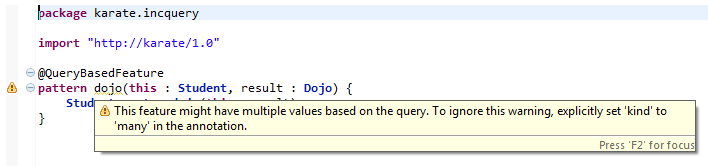
\includegraphics[width=0.9\textwidth]{figures/func-dep-many-warning.png}
\caption{Multiplicitás eltérésre figyelmeztető üzenet}
\label{fig:funcDepManyWarning}
\end{figure}

%----------------------------------------------------------------------------

\section{Lekérdezés teljesítményének javítása}
\label{sect:caseStudy}

Az EMF-IncQuery keresőmotorja egy minta illesztésekor a mintát kielégítő változók egy relációját, egy értéktáblázatot készít el.
Az ilyen relációkat, a relációs adatbázisok működéséhez hasonlóan, általában több kisebb reláció egymáshoz \emph{illesztésével} (join) képzi.
A relációs adatbázisok fejlesztése során már rájöttek, hogy sok múlik ezeknek a műveleteknek a teljesítményén, ezért sok heurisztikát fejlesztettek ki az illesztések lehető leggyorsabb végrehajtásának biztosítására.
Az EMF-IncQuery lekérdezéstervezője is alkalmaz ilyen heurisztikákat, melyek segítségével eldönti, hogy egyáltalán szükséges-e két reláció illesztése, illetve az illesztések mely sorrendje mellett lesz a teljesítmény optimális.

Az egyik ilyen heurisztika a funkcionális függőségeken, pontosabban a funkcionális függőség mentén történő \emph{veszteségmentes felbontás tételén} -- más néven Heath tétele -- alapszik.
A tétel kimondja, hogy ha egy $U$ attribútumhalmaz feletti relációra ($R(U)$) teljesül az $X \rightarrow Y$ függés (ahol $X$ és $Y$ attribútumhalmazok és $XY \subset U$), akkor a relációt e függés mentén felbonthatjuk két másik relációra ($R_1 = \pi_{XY}(R)$ és $R_2 = \pi_{XZ}(R)$, ahol $Z = U \setminus XY$, $\pi$ pedig a vetítés művelete) úgy, hogy a kapott relációk természetes illesztésével visszakapjuk az eredeti relációt ($R = R_1 \bowtie R_2$).
Általános esetben két reláció ($R_1$, $R_2$) illesztésével kapott reláció igen nagy elemszámú lehet.
Legrosszabb esetben az eredményül kapott reláció az alaprelációk Descartes-szorzata, amikor is a kapott reláció elemszáma a két alapreláció elemszámának szorzata: ha $R = R_1 \bowtie R_2 = R_1 \times R_2$, akkor $|R| = |R_1|\cdot|R_2|$.
Ha azonban a két alaprelációra teljesül Heath tétele, akkor az illesztésükkor kapott reláció elemszáma biztosan legfeljebb annyi, mint az alaprelációk elemszámának maximuma.
Ha az ilyen, kisebb elemszámú relációt eredményező illesztéseket előnyben részesítjük, és előbb hajtjuk végre, akkor a fennmaradó illesztések eleve kisebb elemszámú relációkon fognak végrehajtódni, így csökkenthető a végrehajtás erőforrásigénye.

Az EMF-IncQuery fejlesztői által írt lekérdezéstervező a Heath-tételen alapuló heurisztikához az előző szekcióban tárgyalt, általam készített funkcionális függőség elemző függvénykönyvtárat használja.

A heurisztika teljesítményjavító hatását az EMF-IncQuery keretrendszer bemutatásához és teljesítményének méréséhez használt egyik domén-modellen, a \emph{Network} modellen\footnote{\raggedright Forrás: \url{https://github.com/ujhelyiz/EMF-IncQuery-Examples/tree/master/network} (2014.05.24.)} (\ref{fig:EcoreMetaModelExample}. ábra) szeretném bemutatni.
A modellhez három példánymodell készült: egy kicsi (1000 Person, 1000 Post és minden Person-höz 2 Circle), egy közepes (1000 Person, 1000 Post és minden Person-höz 10 Circle) és egy nagy (2000 Person, 2000 Post és minden Person-höz 20 Circle).

A modellhez írt lekérdezések egyike a \ref{lst:mutualFriendsPattern}. kódlistán\footnote{\raggedright Forrás: \url{https://github.com/ujhelyiz/EMF-IncQuery-Examples/blob/master/network/network.incquery/src/network/querySandbox.eiq} (2014.05.24.)} látható.
\begin{lstlisting}[float,floatplacement=htb,caption=MutualFriends minta,label=lst:mutualFriendsPattern]
package network

import "http://network/1.0"

pattern MutualFriends(person: Person, friend: Person) = {
	person != friend;
	Person.circles.members(person, friend);
	Person.circles.members(friend, person);
}
\end{lstlisting}
Ennek a lekérdezésnek az egyik sajátossága, hogy naiv módszerrel történő kiértékelése rengeteg illesztési műveletet igényel, és eközben nagy elemszámú relációkat hoz létre.

Az EMF-IncQuery Java virtuális gépen fut, így annak automatikus memóriakezelését használja -- a szemétgyűjtés módszerét (garbage collection).
A szemétgyűjtő működésének elve, hogy periodikusan vagy memóriahiány esetén megkísérli felszabadítani a memóriának azt a részét, amelyet az alkalmazás már nem használ.
Ha a program gyakran foglal le sok memóriát és azt csak rövid ideig használja, akkor a szemétgyűjtőnek gyakran kell lefutnia, hogy ki tudja elégíteni az alkalmazás újabb és újabb memóriaigényeit.
 
Méréseim során a közepes és a nagy példánymodelleken a fenti lekérdezés a Heath tételén alapuló heurisztika nélkül valamivel több, mint 4GB maximális memóriahasználat engedélyezésével sem futott le sikeresen egy-két órán belül.
A heurisztika engedélyezése után a közepes példánymodellen átlagosan 3 másodperc alatt futott le a lekérdezés, amihez 0,5GB memóriát használt fel. A nagy példánymodellen a lekérdezés átlagosan 16 másodperc alatt futott le és 1,5GB memóriát igényelt.
A mérések természetesen különböző hardvereken eltérőek lehetnek, ám az elért teljesítménynövekedés egyértelmű.
